% =====================================================================
% Rolling-Governed Pinch Stability — RA-L submission
% Source of truth: this file (paper/main.tex). Markdown drafts:
% ../PAPER.md (draft 1), ../PAPER_v2.md (draft 2, ported here).
% Compile: tectonic main.tex   (or latexmk -pdf main.tex / Overleaf)
% =====================================================================
\documentclass[journal]{IEEEtran}

\usepackage{graphicx}
\usepackage{amsmath,amssymb}
\usepackage{booktabs}
\usepackage[hidelinks]{hyperref}
\usepackage{balance}

\newcommand{\mueff}{\mu_{\mathrm{eff}}}
\newcommand{\mupair}{\mu_{\mathrm{pair}}}
\newcommand{\fstar}{f^{*}}
\newcommand{\repourl}{\url{https://github.com/NutcrackerWOW/Simplified-3D-Object-Manipulation-using-TacTip}}

\begin{document}

\title{Rolling Governs Pinch Stability for Soft Tactile Fingertips:\\
  A Simulation Study of the Minimal Grip-Force Window}

\author{Jinxi Chen%
  \thanks{Manuscript received 06/07/2026; revised XXX. (Corresponding author:
    Author Name.)}%
  \thanks{The author is with Bristol Robotics Laboratory (e-mail: jinxichenhhh@gmail.com).}%
  \thanks{Code, models, and data are released at
    \protect\repourl.}%
}

\markboth{IEEE Robotics and Automation Letters. Preprint version.}%
{Jinxi Chen: Rolling-Governed Pinch Stability}

\maketitle

\begin{abstract}
Soft optical tactile fingertips such as the TacTip gain their sensitivity
from compliance, but the same compliance lets a pinched object \emph{roll}
off the fingertip domes below the Coulomb sliding limit. Rolling-based
pinch controllers exploit that freedom to reach equilibrium at a
\emph{commanded} squeeze force, but leave open how small that command may
safely be. In a simulation study (Drake, compliant-hydroelastic contact) of
a two-finger pinch with TacTip-style domes, we measure the minimal stable
squeeze force $\fstar$ --- the floor of the commanded-force window ---
across grasp posture, object mass, shape, friction, and fingertip
stiffness. The stability boundary is rolling-governed: the effective
stability ratio $\mueff = (mg/2)/\fstar$ sits 25--35\,\% below the pair
Coulomb coefficient at every friction tested, so a friction-cone analysis
systematically underestimates the required force. Shape alone spans a
$2\times$ range of $\fstar$ at fixed friction, ordered by the object's
freedom to roll, and softer solid-dome fingertips reduce $\mueff$
($0.68 \to 0.49$, $100 \to 25$~kPa). Bootstrap analysis shows $\mueff$ is
statistically flat in posture inside the validity envelope; for this
testbed the calibration is $\mueff \approx 0.71 - 4.2\,(m - 0.045)$ [$m$ in
kg], passing 16/16 held-out posture--mass probes --- the coefficients are
testbed-specific, the functional form and fitting protocol are the
contribution. Near the boundary, grasps fail by slow rolling creep with no
vibration warning; the failure times are insensitive to solver time step,
contact dissipation, and friction regularization, motivating a
$\times 2.0$ force margin under which 30/30 seeded carry runs succeed.
Closing the loop on the rolling degree of freedom itself --- a simplified
rolling-orientation regulator driven by contact-centroid migration ---
arrests the creep (10/10 vs.\ 0/20) and lowers the sustained-hold
requirement to ${\approx}1.15\times\fstar$ while leaving the boundary
unmoved: the rolling discount is geometric, but the duration penalty is
controllable. A posture-scheduled threshold also makes a vibration slip
detector usable at the sensor's 100~Hz camera rate. Code and data are
publicly released.
\end{abstract}

\begin{IEEEkeywords}
Grasping, force and tactile sensing, contact modeling, simulation and
animation, grippers and other end-effectors.
\end{IEEEkeywords}

\IEEEpeerreviewmaketitle

\section{Introduction}

\IEEEPARstart{G}{rip} force selection is the most basic decision a
manipulating hand makes: squeeze too little and the object falls, squeeze
too much and the object is deformed, ejected, or energy is wasted. Sixty
years of grasp analysis provide the standard answer --- treat each contact
as a friction cone, require the load wrench to be resisted inside the
cones, and add an empirical safety margin. For rigid point contacts this is
essentially correct. But modern tactile fingertips are not rigid points:
sensors such as the TacTip family
\cite{chorley2009development,wardcherrier2018tactip} wrap a soft
hemispherical membrane around a camera, and the same compliance that gives
them their sensitivity gives the grasped object a new way to fail --- it
can \emph{roll} off the dome.

This paper quantifies that failure mode and turns the result into an
engineering rule. We build a simulation testbed around a two-finger hand
with compliant hydroelastic fingertip domes, pinching gravity-loaded
objects with the pinch axis horizontal so that weight loads the contacts in
shear (Fig.~\ref{fig:setup}). Because the testbed measures the
\emph{acquisition-to-hold} pipeline end to end --- close, grip, release,
hold --- we can locate the minimal stable squeeze force $\fstar$ by
bisection for any posture, object, and material, and ask what actually sets
it.

The answer is consistent across every sweep we ran: the boundary is
\textbf{rolling-governed}. At forces just below $\fstar$ the object does
not slide down the pads; it rotates about the grasp axis and escapes
(Fig.~\ref{fig:rolling}). The effective stability ratio
$\mueff = (mg/2)/\fstar$ --- the number a Coulomb analysis would call
``friction being used''; higher $\mueff$ means a cheaper-to-hold grasp ---
saturates 25--35\,\% below the material pair's Coulomb coefficient at every
tested friction level, and a shape study at constant mass and friction
spans a $2\times$ range of $\fstar$ ordered exactly by rolling freedom
(Fig.~\ref{fig:shapes}). None of this is visible to a friction-cone
analysis, which predicts the same force for a sphere and a disc.

The number this map produces has a specific consumer. A line of
soft-fingertip pinch control running from the dual soft-tip finger
dynamics of Arimoto et al.\ \cite{arimoto2000dynamics,arimoto2008control}
to rolling-orientation control \cite{psomopoulou2018stable} and its
TacTip-hardware realization \cite{psomopoulou2021pinching} treats rolling
as a \emph{resource}: the fingertips are actively rolled to reach a stable
equilibrium at a \emph{commanded} squeeze force. That theory takes the
commanded force as an input --- friction adequacy is an assumption in the
proofs, not a computed quantity --- and does not say how small the command
may safely be. This paper measures exactly the piece the theory leaves
open: for which commanded forces the pinch equilibrium exists and
persists. The answer is a \emph{window} --- roll-out from below, ejection
from above --- whose floor sits 25--35\,\% above what friction analysis
predicts. Those controllers answer how to reach the equilibrium and stay
there; our map answers how hard one must squeeze for that equilibrium to
exist at all. The rule below is the set-point law for that class of
controllers.

Rolling failure of soft contacts is not new \emph{qualitatively} --- the
kinematics of rolling contact are classical \cite{montana1988kinematics},
the soft-finger contact model and its limit surface
\cite{goyal1991planar,kao1992quasistatic,xydas1999modeling} bound the
coupled force--torque capacity of a compliant patch, rolling of deformable
fingertips has explicit kinematic models \cite{doulgeri2003grasping}, the
elastic-energy view identifies the restoring moment a soft tip exerts
about its equilibrium \cite{inoue2006elastic}, and rotational stability
conditions have recently been derived for soft pneumatic fingers
\cite{jang2024rotational}. Our contribution is \emph{quantitative and
operational}: we measure where the boundary actually lies for a realistic
soft-fingertip geometry across posture, mass, shape, friction, and
stiffness; we identify the regimes where the friction picture breaks
entirely (a geometric support regime, a fragile seed-dependent band, a
squeeze-out ejection ceiling, and a mass ceiling where the stable window
closes); and we compress the result into a one-line minimal-force
calibration with a stated envelope, tested on held-out conditions.

Contributions:
\begin{enumerate}
  \item \textbf{Mechanism, quantified.} Across shape, friction, and
    stiffness sweeps, the pinch stability boundary for soft hemispherical
    fingertips is set by rolling, not Coulomb sliding: $\mueff$ sits
    25--35\,\% below the pair friction at all tested frictions; geometry
    alone moves $\fstar$ by $2\times$ at fixed friction; and softer
    fingertips lower $\mueff$, from 0.68 at 100~kPa to 0.49 at 25~kPa,
    exposing a direct sensitivity-versus-stability trade-off in soft
    tactile sensor design.
  \item \textbf{A minimal grip-force calibration with a stated envelope.}
    $f_1^{*} = (mg/2)/\mueff$ with the one-line
    $\mueff \approx 0.71 - 4.2\,(m-0.045)$ for this testbed: bootstrap
    confidence intervals show the boundary is statistically flat in
    posture inside the validity envelope, so mass --- not posture ---
    carries the rule, with a fitted quadratic posture refinement and
    automatically classified failure regimes reported alongside. The rule
    scores 16/16 on held-out posture--mass probes (hold at $1.25\times$
    prediction, drop at $0.6\times$). The coefficients are specific to
    this hand, material pair, and grasp width; the transferable
    contribution is the functional form and the bisection-plus-fit
    protocol that recalibrates it on any other testbed.
  \item \textbf{Slip-threshold calibration that survives scale, at the
    sensor's camera rate.} On a 90-episode study spanning the envelope, the pre-slip
    vibration floor varies up to $72\times$ across conditions, so any
    single global threshold fails (0/30 detections at the only safe
    setting) even though every slip burst clears its own condition's floor
    by ${\ge}3.6\times$. Scheduling the threshold over $(\phi,\theta,m)$
    --- the same recipe that schedules grip force --- recovers
    30~TP\,/\,1~FP\,/\,0~FN\,/\,29~TN at both the ideal rate and the
    100~Hz camera rate.
  \item \textbf{The first measurement of what rolling regulation buys in
    minimal grip force.} A simplified rolling-orientation regulator ---
    differential PIP flexion driven by the antisymmetric migration of the
    two contact centroids, a tactile-only signal --- arrests the
    margin-1.3 rolling creep (10/10 held vs.\ 0/20 open-loop), lowers the
    sustained-hold requirement from $\times 2.0$ to
    ${\approx}\times 1.15\,\fstar$, and leaves the 3~s acquisition
    boundary unchanged ($-3$ to $+7$\,\%): the static rolling discount is
    geometric, the hold-duration penalty is a controllable artifact of
    leaving the rolling DOF open-loop (\S\ref{sec:closedloop}).
\end{enumerate}

We also show the measured boundary is \textbf{hold-duration-dependent}: at
$1.3\times\fstar$ the grasp survives the classic 3~s test window but fails
within 4--10~s of hold by slow rolling creep, with no detectable difference
between motionless and carried holds (\S\ref{sec:carried}), and with
failure times insensitive to solver time step, contact dissipation, and
friction-regularization tolerance. Rolling creep produces
almost no tangential vibration until roll-off is imminent, so no reflex can
save a grasp commanded at that margin --- the $\times 2.0$ margin in our
rule is not conservatism but a measured requirement for sustained holds.

The study is simulation-only by design, and its products are scoped
accordingly: a mechanism map (which failure channel binds, where), a
calibration recipe (the protocol that refits the rule on any testbed), and
a hardware-validation roadmap. Hydroelastic contact gives us a controlled,
converged testbed in which $\fstar$ is measurable to a few percent, every
failure is replayable, and 2{,}100-trial sweeps are tractable; the
headline temporal result is additionally checked against the contact
model's own dissipative and regularization parameters
(\S\ref{sec:carried}). Hardware transfer --- replacing the idealized
contact resultant with real TacTip marker flow, with its noise,
hysteresis, and calibration error \cite{lepora2021soft} --- is future
work, and \S\ref{sec:limitations} details what the idealization does and
does not cover.

\section{Related Work}

\textbf{Soft-finger contact and limit surfaces.} The soft-finger contact
model augments point friction with torsional resistance over a finite
patch; the limit-surface formalism
\cite{goyal1991planar,kao1992quasistatic,xydas1999modeling} bounds the
coupled tangential-force/torque capacity and predicts that torque demand
reduces tangential capacity, and under viscoelastic contact that capacity
\emph{relaxes} under sustained load \cite{tiezzi2007modeling} --- the
literature's closest analogue of the hold-duration-dependent boundary we
measure in \S\ref{sec:carried}. That fingertip material and geometry
choices set grasp stability is a design axis identified four decades ago
\cite{cutkosky1986friction}; our stiffness sweep places TacTip-style solid
domes on it quantitatively. Closest in spirit, Jang et al.\
\cite{jang2024rotational} derive an analytical rotational-stability
condition for soft-finger precision grasps from bulk finger stiffness,
validated on pneumatic fingers. Our measurements are consistent with that
line and go beyond it in two ways: the failing rotation here is about
the \emph{grasp axis} (the object rolls over the dome's curvature, a
geometric escape rather than in-patch spin \cite{montana1988kinematics}),
and we measure the resulting boundary as a scalar field
$\mueff(\phi,\theta,m)$ --- spanning friction, shape, tip stiffness, and
hold duration --- rather than a per-contact constitutive model or a
per-finger stiffness condition. In the standard taxonomy
\cite{bicchi2000robotic}, what we map is the existence region of a
force-closure equilibrium for a rolling-dominant contact pair.

\textbf{Grip force control and margins.} Human studies
\cite{johansson1984roles,johansson2009coding} established that people
control precision grip as a grip-to-load \emph{ratio} with a small
scheduled safety margin, updated by tactile slip events. Our rule
rearranges to exactly that form --- grip force $= (2/\mueff) \times$ load
force --- with a rolling-discounted $\mueff$ where humans use their
slip-referenced friction estimate. Robotic equivalents estimate the
friction coefficient or slip margin online from tactile signals, from early
skin-acceleration slip sensing \cite{howe1989sensing} to recent soft-finger
Coulomb-state estimation from tactile arrays \cite{jang2024soft}. These
approaches presume the operative limit is frictional and \emph{estimate}
where it lies; we instead measure that for soft domes the operative limit
is rolling, sits 25--35\,\% below the frictional one, and --- near the
boundary --- moves with hold duration, and we \emph{prescribe} the
resulting minimal force in the carefully-scoped empirical-contact-model
register of \cite{howe1996practical}. Margins calibrated against Coulomb
slip are optimistic in exactly the regime where they matter. For TacTip
fingertips specifically, Psomopoulou et al.\ \cite{psomopoulou2021pinching}
stabilize a two-finger pinch by actively \emph{rolling} the tips to an
equilibrium at a commanded squeeze force --- rolling as a control
resource; our rule supplies the minimal admissible value of that
commanded force, treating the same rolling freedom as the failure channel
that sets it (\S\ref{sec:envelope}); \S\ref{sec:closedloop} measures what
regulating that freedom buys back.

\textbf{Slip detection with optical tactile sensors.} Vibration- and
flow-based slip detection is well established for TacTip
\cite{chorley2009development,wardcherrier2018tactip,james2018slip} and
GelSight-class sensors \cite{johnson2009retrographic,yuan2017gelsight};
James and Lepora \cite{james2021slip} close the loop on hardware, with
detected slip triggering grip response on a multifingered TacTip hand ---
the closest benchmark for \S\ref{sec:slip}. For a survey of tactile
sensing in dexterous hands see \cite{kappassov2015tactile}. Reported
detectors are typically evaluated at one or few conditions. Our expanded study reproduces the common
single-condition success and then shows the cross-condition calibration
problem ($72\times$ floor variation) that a deployment must solve; the
proposed fix (threshold scheduling over posture and load) uses no
additional sensing.

\textbf{Simulation of compliant contact.} We rely on Drake's
compliant-hydroelastic contact model with the SAP discrete solver
\cite{elandt2019pressure,masterjohn2022velocity,castro2023unconstrained},
which produces continuous pressure-field contact wrenches for soft
geometries and is a current standard for contact-rich manipulation
simulation. Its dissipation term is of the Hunt--Crossley family, whose
modeling assumptions and limits are analyzed in \cite{marhefka1999compliant}.
Tactile simulators in the same spirit have demonstrated
sim-to-real transfer for TacTip-class sensors \cite{lin2022tactilegym2},
which is the intended path for the hardware validation discussed in
\S\ref{sec:limitations}. We verify our headline temporal result (creep
failure time) is converged across $2\times$--$4\times$ time-step
refinement and insensitive to the contact model's dissipation and
friction-regularization parameters (\S\ref{sec:carried}).

\section{Simulation Testbed}
\label{sec:testbed}

\begin{figure*}[t]
  \centering
  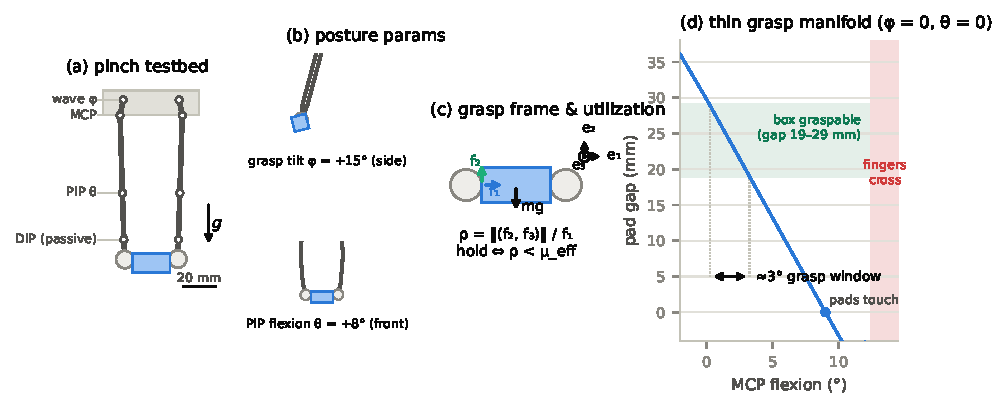
\includegraphics[width=\textwidth]{figs/F1_setup.pdf}
  \caption{Simulation testbed. (a)~Two-finger hand with compliant
    hydroelastic fingertip domes, mounted fingers-down so gravity loads the
    pinch contacts in shear. (b)~The two posture parameters: grasp tilt
    $\phi$ rigidly rotates the grasp about the pinch axis (reorienting
    gravity on the pads); PIP flexion $\theta$ re-bends the fingers at
    fixed pad gap. (c)~Grasp frame built from the two contact
    centroids: squeeze $f_1$, weight-bearing shear $f_2$, lateral shear
    $f_3$; utilization $\rho = \lVert(f_2,f_3)\rVert / f_1$. (d)~The grasp
    manifold is thin: the pad gap sweeps its graspable band in
    ${\approx}3^\circ$ of MCP flexion, so postures are parameterized by
    $(\phi, \theta)$ with MCP solved per condition.}
  \label{fig:setup}
\end{figure*}

\textbf{Hand and materials.} The testbed (Fig.~\ref{fig:setup}a) is a
two-finger hand (``Touch\_Finger'') with per-finger kinematic chain
wave~$\to$~MCP~$\to$~PIP~$\to$~DIP, mounted fingers-down so the pinch axis
is horizontal and gravity loads the contacts in shear. Wave, MCP, and PIP
are actuated (posture PD with gravity feedforward); DIP is passive, a
torsional spring toward the measured PIP angle (k = 0.35~N$\cdot$m/rad,
${\approx}5^\circ$ of give at 1--2~N), mimicking the compliance of a distal
pad mount. Fingertips are hemispherical domes simulated as compliant
hydroelastic solids (elastic modulus 50~kPa nominal,
$\mu_s/\mu_d = 1.2/0.9$); objects are rigid hydroelastic
($\mu_s/\mu_d = 1.0/0.8$), giving a Coulomb pair coefficient
$\mu_d \approx 0.85$ (harmonic mean). The reference object is a
$25 \times 25 \times 12$~mm, 50~g block. Simulation uses Drake~1.54, SAP
solver (\texttt{kSap} discrete approximation), 2~ms steps for boundary
trials and 1~ms for slip trials. Under \texttt{kSap}, contact dissipation
is the linear Kelvin--Voigt model with relaxation time $\tau$ (Drake
default 0.1~s per geometry) and friction is regularized in impulse space
(dimensionless $\sigma = 10^{-3}$); a Hunt--Crossley dissipation of
1.5~s/m is additionally declared on the tips and is consumed by the
alternative \texttt{kLagged}/\texttt{kSimilar} approximations used in the
solver-sensitivity study of \S\ref{sec:carried}, which varies $\tau$, the
Hunt--Crossley dissipation, the friction-regularization tolerance, and
the contact approximation itself.

\textbf{Idealized tactile signal.} Per fingertip we read the hydroelastic
contact resultant force and patch centroid --- an idealized TacTip. From
the two centroids we build the grasp frame (Fig.~\ref{fig:setup}b): $e_1$
along the grasp axis (squeeze force $f_1$), $e_2$ vertical in the plane
normal to $e_1$ (the weight-bearing shear $f_2$),
$e_3 = e_1 \times e_2$ (lateral shear $f_3$). Utilization
$\rho = \lVert (f_2, f_3) \rVert / f_1$ is the fraction of a Coulomb budget
in use; classical analysis predicts failure at $\rho \approx \mupair$.
Sensor-rate realism is covered by evaluating the slip detector on a 100~Hz
sample-and-hold variant of the signal, the camera rate of the physical
sensor.

\textbf{Grasp acquisition and force control.} A state machine closes to a
posture, acquires contact, servos the squeeze component $f_1$ to a setpoint
(integral torque trim on MCP), releases the object's spawn support, and
holds. Gravity-compensation feedforward on the actuated joints is required
at tilted postures --- without it, PD sag consumes the few-degree contact
window.

\textbf{The grasp manifold is thin.} The pads oppose ${\sim}30$~mm apart at
zero flexion and the fingers physically cross a few degrees later
(Fig.~\ref{fig:setup}c): the pad gap sweeps its full graspable band in
${\approx}3^\circ$ of MCP flexion. Grasp postures are therefore
parameterized by \textbf{grasp tilt $\phi$} ($\pm 15^\circ$; opposite wave
values on the two fingers, a rigid rotation of the grasp about the pinch
axis that reorients gravity on the pads) and \textbf{PIP flexion $\theta$}
($-5^\circ \ldots +10^\circ$), with MCP solved per condition to hit a 24~mm
pad gap.

\textbf{Boundary protocol.} For each condition $(\phi,\theta,\mathrm{mass})$
the minimal stable squeeze $\fstar$ is located by a mass-scaled ascending
force ladder followed by log-space bisection: 7 steps, 2 spawn seeds per
probe (a probe is stable only if \emph{all} seeds hold), ``stable'' =
object drift $< 2$~mm in the tip frame over a 3~s hold. The primary sweep
covers 5 tilts $\times$ 8 flexions $\times$ 3 masses (30/60/120~g) = 120
conditions, ${\approx}2{,}100$ trials. Three dedicated studies use stronger
statistics: shape/material tables use 5 seeds per probe, the carried-grasp
failure statistics use 10 seeds per condition, and a seed-noise audit (12
conditions $\times$ 5 independent single-seed bisections) measures the
seed-to-seed spread of $\fstar$ itself --- 2--7\,\% of the median at 30~g
(the bisection notch) but 7--32\,\% at 60~g, numbers that become the
weights and exclusions of \S\ref{sec:envelope}.

\section{The Stability Boundary Is Rolling-Governed}
\label{sec:rolling}

\begin{figure*}[t]
  \centering
  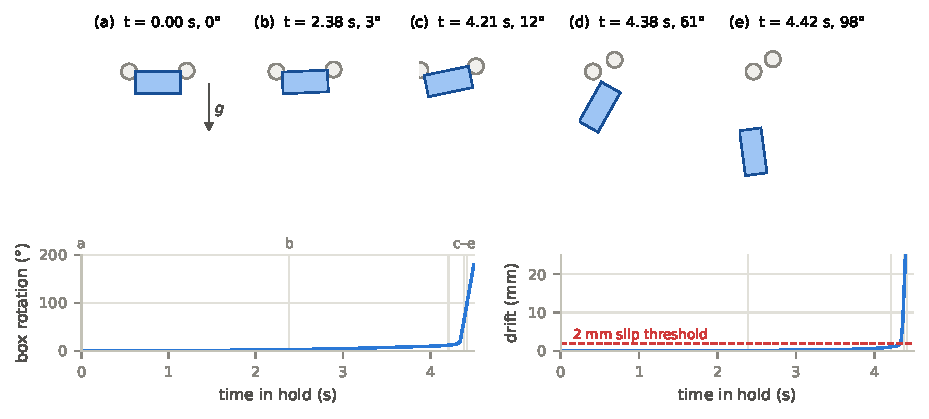
\includegraphics[width=\textwidth]{figs/F2_rolling.pdf}
  \caption{Anatomy of the canonical failure: a 50~g block held at
    $1.3\times\fstar$ (all times from hold start). (a--e)~Snapshots
    through the creep and roll-off. (f)~Both failure coordinates
    normalized by their own criterion: rotation spends its budget while
    drift idles at a quarter of its 2~mm threshold until roll-off.
    (g)~The contact interface itself: relative tangential speed at both
    contacts stays an order of magnitude below the 5~mm/s sliding
    criterion through the creep --- the interface is in stick while the
    patch migrates (rolling) --- and breaks only in the final
    ${\sim}0.3$~s. At failure, utilization $\rho \approx 0.5$: barely
    half the nominal friction budget is in use.}
  \label{fig:rolling}
\end{figure*}

\textbf{Failure looks like rolling, everywhere.} Fig.~\ref{fig:rolling}
shows the canonical failure: a 50~g block held at $1.3\times\fstar$ at the
reference posture (times are measured from hold start; the
acquisition sequence takes ${\approx}1.2$~s before it). For over four
seconds the grasp looks quiet --- drift under a millimeter --- while the
block rotates at degrees per second about the lateral axis. The rotation
accelerates smoothly, the block rolls over the dome shoulders, and it is
gone ${\sim}200$~ms later, tumbling $176^\circ$ before free fall.
Translation (the thing a Coulomb analysis watches) stays below the 2~mm
threshold until the roll-off is already unrecoverable. At failure,
utilization $\rho \approx 0.5$: the grasp ``uses'' barely half its nominal
friction budget when it dies.

\textbf{The interface sticks while the object rotates.} The rolling claim
is directly observable at the contact (Fig.~\ref{fig:rolling}, bottom
right): through the 4~s creep phase the relative tangential speed at both
contacts stays below 3~mm/s --- under the 5~mm/s kinematic sliding
criterion, with the left interface in essentially perfect stick
(integrated interfacial slip 0.03~mm over 4~s, against the
${\approx}2$~mm it would need if the observed $10^\circ$ of rotation
were produced by sliding). Meanwhile both contact centroids migrate
0.4--0.9~mm down the domes: the rotation is carried by the patch
\emph{migrating} over the dome --- rolling --- not by interfacial
sliding. Only in the final ${\sim}0.3$~s does the interface break to
$10^1$--$10^2$~mm/s as the block rolls off.

\textbf{The stability ratio never reaches Coulomb.} Define
$\mueff = (mg/2)/\fstar$, the value a friction-cone analysis would infer
from the measured boundary; higher $\mueff$ means less force is needed ---
a better grasp. If sliding governed, $\mueff$ would equal the pair
coefficient. Instead, across the friction sweep (box object, reference
posture, Table~\ref{tab:materials} and Fig.~\ref{fig:shapes}b),
$\mueff/\mupair$ stays at 0.66--0.77 in the mid-to-high friction range:
$\fstar$ follows the Coulomb-like $1/\mu$ scaling --- friction sets the
\emph{scale} --- but the boundary binds 25--35\,\% early, at the roll-off.

\begin{table}[t]
  \caption{Material study: friction pair and fingertip stiffness (box
    object, reference posture, 5 seeds).}
  \label{tab:materials}
  \centering
  \setlength{\tabcolsep}{4pt}
  \resizebox{\columnwidth}{!}{%
  \begin{tabular}{lcccc}
    \toprule
    material variation & pair $\mu_d$ & $\fstar$ (N) & $\mueff$ &
      $\mueff/\mupair$ \\
    \midrule
    low friction (box $\mu_d$ 0.3) & 0.45 & \multicolumn{3}{c}{none ---
      window closed} \\
    base (box $\mu_d$ 0.8) & 0.85 & 0.435 & 0.564 & 0.66 \\
    high friction (box $\mu_d$ 1.2) & 1.03 & 0.311 & 0.789 & 0.77 \\
    soft tips, 25~kPa & 0.85 & 0.504 & 0.487 & 0.57 \\
    stiff tips, 100~kPa & 0.85 & 0.360 & 0.681 & 0.80 \\
    \bottomrule
  \end{tabular}}
\end{table}

\begin{table}[t]
  \caption{Shape study: geometry only (50~g, identical friction pair,
    25~mm grasp width, 5 seeds).}
  \label{tab:shapes}
  \centering
  \setlength{\tabcolsep}{4pt}
  \resizebox{\columnwidth}{!}{%
  \begin{tabular}{llcc}
    \toprule
    shape & contact type & $\fstar$ (N) & $\mueff$ \\
    \midrule
    disc, axis $\parallel$ grasp axis & flat round faces & 0.298 & 0.823 \\
    box $25{\times}25{\times}12$~mm & flat square faces & 0.435 & 0.564 \\
    prism $25{\times}50{\times}12$~mm & flat faces, $2\times$ lever arm &
      0.435 & 0.564 \\
    cylinder $d=25$~mm, axis vertical & curved rim & 0.464 & 0.529 \\
    disc on edge (key pinch) & rim, gravity on roll axis & 0.572 & 0.429 \\
    sphere $d=25$~mm & point contact & 0.596 & 0.411 \\
    \bottomrule
  \end{tabular}}
\end{table}

\begin{figure}[t]
  \centering
  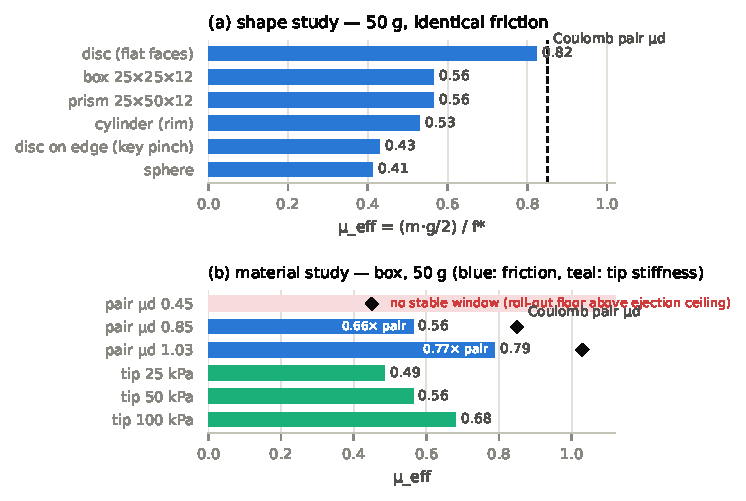
\includegraphics[width=\columnwidth]{figs/F3_shapes_materials.pdf}
  \caption{(a)~Shape study: $\mueff$ ordered exactly by the object's
    freedom to roll, spanning $2\times$ in $\fstar$ at identical Coulomb
    friction. (b)~Material study: $\mueff$ tracks but never reaches the
    pair coefficient (rolling discount $0.66$--$0.77$); softer tips are
    worse.}
  \label{fig:shapes}
\end{figure}

\begin{figure*}[t]
  \centering
  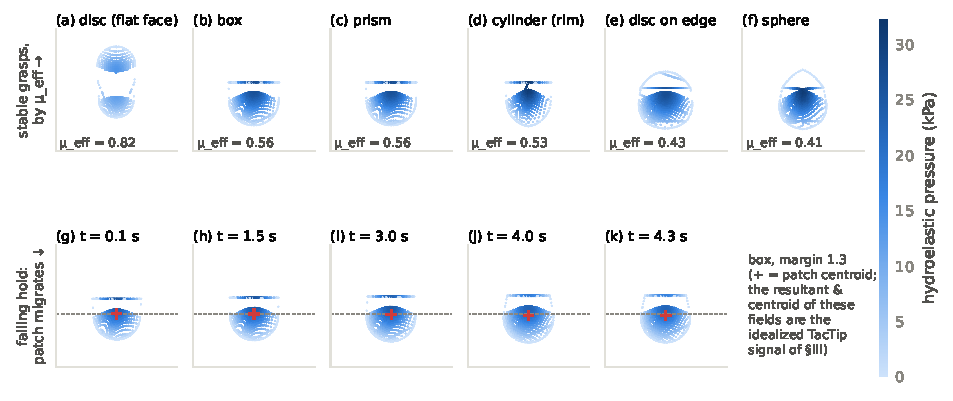
\includegraphics[width=\textwidth]{figs/F9_patches.pdf}
  \caption{The contact patches behind the numbers. Top row: hydroelastic
    pressure field on the L-tip contact for each shape-study object in the
    reference grasp (at $1.25\times$ its own $\fstar$), ordered by
    $\mueff$: the broad flat-face patch with its long restoring lever arm
    shrinks toward the sphere's near-point contact. The resultant and
    centroid of exactly these fields are the idealized TacTip signal of
    \S\ref{sec:testbed}. Bottom row: the box's L-tip patch through a
    failing margin-1.3 hold --- the patch (centroid $+$) migrates over
    the dome shoulder as the block rolls; dashed line marks the initial
    centroid height.}
  \label{fig:patches}
\end{figure*}

\textbf{Geometry alone spans $2\times$ at fixed friction.} The shape study
(Fig.~\ref{fig:shapes}a, Table~\ref{tab:shapes}) holds mass (50~g),
friction pair, and grasp width (25~mm) fixed and varies only geometry. The
ordering is exactly the object's freedom to roll in the grasp
(Fig.~\ref{fig:patches}, top row): flat faces
pressed by domes resist rotation best; rims and points roll easily; lateral
prehension of a disc is nearly worst because gravity torque acts directly
about the free rolling axis. Two details sharpen the mechanism. First, box
and prism land on \emph{exactly} the same bisection notch
($\fstar = 0.435$~N at 5-seed resolution): doubling the lever arm about the
grasp axis changes nothing, so the flat-face boundary is set by the contact
patch, not the object's inertia. Second, the span disc~$\to$~sphere is
$2.0\times$ in $\fstar$ --- larger than the entire friction effect over the
tested range --- at \emph{identical} Coulomb friction. No friction-cone
analysis, however carefully calibrated, can reproduce this column.

\textbf{Softer fingertips are worse.} The naive expectation --- softer pad,
larger patch, more rolling resistance --- fails in the direction that
matters for sensor design: $\mueff$ falls from 0.68 (100~kPa) to 0.56
(50~kPa) to 0.49 (25~kPa). A compliant dome yields as the object rotates
and provides less restoring moment against rolling, so the skin softness
that maximizes tactile sensitivity directly taxes grasp stability. For
TacTip-class sensors this is a quantified design trade-off, not a
qualitative caution. Its scope is \emph{solid} elastic domes --- the
honest boundary of this testbed: a physical TacTip is a thin membrane over
a gel with pins, whose rolling resistance comes from skin tension and
internal pressure rather than bulk elasticity \cite{lepora2021soft}, and
membrane tips exhibit hysteresis and viscoelasticity a solid
Hunt--Crossley dome cannot reproduce. Whether the ordering transfers to
membrane construction is a question for the hardware follow-up
(\S\ref{sec:limitations}).

\textbf{The friction picture can collapse entirely.} At pair
$\mu_d = 0.45$ the hold boundary (roll-off from below, 0.74~N) rises past
the ejection boundary (squeeze-out from above, ${\ge}1.5$~N at this
friction): the stable window is empty and \emph{no} squeeze force holds a
50~g box. Stability for soft fingertips is a \textbf{window}, not a
threshold --- its ceiling (\S\ref{sec:envelope}) is as real as its floor.

\section{The Stability Envelope and a Minimal Grip-Force Rule}
\label{sec:envelope}

\begin{figure*}[t]
  \centering
  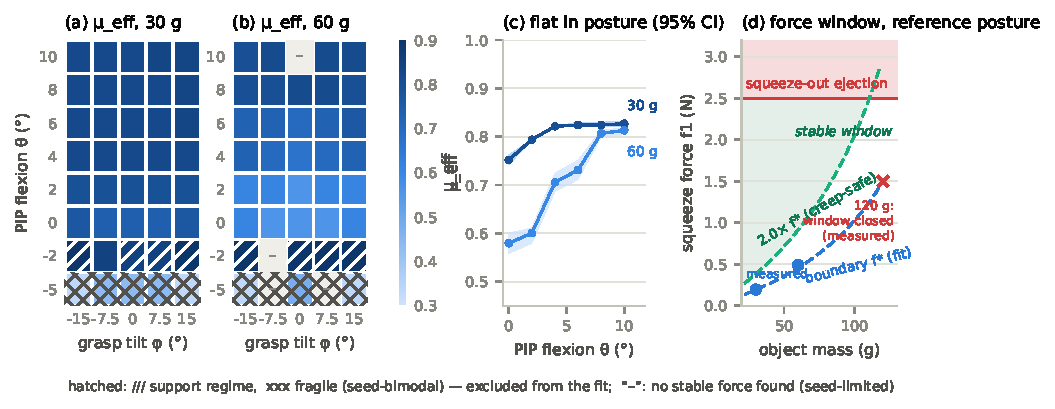
\includegraphics[width=\textwidth]{figs/F4_envelope.pdf}
  \caption{The stability envelope. (a,b)~$\mueff$ maps at 30 and 60~g with
    automatically classified regimes: support band (///, $\fstar$
    mass-independent) and fragile band ($\times\times\times$, boundary
    existence seed-dependent) are excluded from the fit; ``--'' cells:
    no stable force found at 2-seed resolution (seed-limited, cf.\ the
    audit of \S\ref{sec:testbed}). (c)~$\mueff$ vs.\ PIP flexion with
    bootstrap 95\,\% CIs of the across-tilt mean, one line per mass ---
    the flatness claim, shown directly. (d)~The stable force window
    $[\fstar, {\approx}2.5~\mathrm{N}]$ narrows with mass and closes at
    120~g; dots are measured boundaries, curves are the fitted rule
    (dashed: interpolation).}
  \label{fig:envelope}
\end{figure*}

\textbf{The rule.} Inside the validity envelope established below, the
minimal stable squeeze force is
\begin{equation}
  f_1^{*}(m) = \frac{m g / 2}{\mueff}, \qquad
  \mueff \approx 0.71 - 4.2\,(m - 0.045)
  \label{eq:rule}
\end{equation}
with $m$ in kilograms. Mass, not posture, carries the rule. Bootstrap confidence intervals over
the fitted sweep (5{,}000 condition resamples) retain only the intercept
(0.707, 95\,\% CI $[0.674, 0.739]$) and the mass slope ($-4.20$, CI
$[-5.14, -3.20]$); every posture coefficient's CI straddles zero. Inside
the envelope, $\mueff$ is statistically flat in posture
(Fig.~\ref{fig:envelope}c); posture decides
grasp stability at the \emph{regime boundaries} (below), not inside the
safe region. Fig.~\ref{fig:rule} shows the rule against the measured
conditions, its bootstrap uncertainty, and the held-out test below.

\begin{figure}[t]
  \centering
  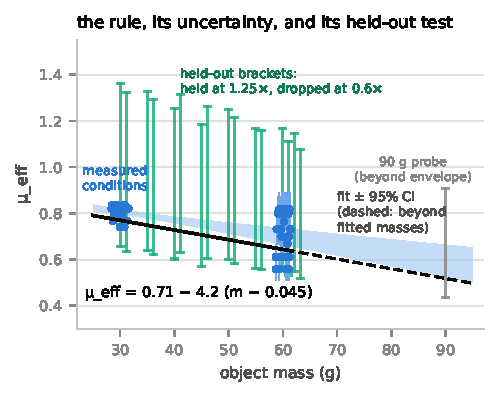
\includegraphics[width=\columnwidth]{figs/F7_rule.pdf}
  \caption{The rule of Eq.~\eqref{eq:rule} against everything that tests
    it: friction-regime conditions at 30/60~g with audit-measured
    seed-noise error bars, the weighted fit with a bootstrap 95\,\% CI
    band, and the 16 held-out probes drawn as brackets
    $[\mueff^{\mathrm{pred}}/1.25,\, \mueff^{\mathrm{pred}}/0.6]$ --- each
    probe held at $1.25\times$ the predicted force and dropped at
    $0.6\times$, so the true boundary lies inside its bracket; the fitted
    line threads all 16. The 90~g bracket is an out-of-envelope probe
    that also passed.}
  \label{fig:rule}
\end{figure}

\textbf{What the coefficients are --- and are not.} Equation~\eqref{eq:rule}
is a calibration for one envelope: this hand, this material pair, one
25~mm grasp width, masses validated over 30--60~g. It is not a law of
nature --- the mass coefficient carries units of kg$^{-1}$, and
extrapolating it far outside the fitted range is meaningless (well before
the fitted line reaches zero, the window itself closes at 120~g,
Fig.~\ref{fig:envelope}d). What transfers is the functional form ---
affine in mass, flat in posture inside the envelope --- and the protocol:
any other hand can rerun the bisection procedure of \S\ref{sec:testbed}
at a handful of masses and refit its own two numbers.

\textbf{Why heavier objects need disproportionately more force.} The
decline of $\mueff$ with mass ($\fstar$ grows by $2.3\times$ when mass
doubles from 30 to 60~g) has a mechanical reading consistent with the
elastic restoring-moment view of soft tips \cite{inoue2006elastic} and
with the failure anatomy of \S\ref{sec:rolling}. The escape channel is
patch migration over the dome shoulder, so the grasp's rotational reserve
is the angular distance between the loaded patch position and the
shoulder. The weight-bearing shear $mg/2$ statically drags the patch
toward the shoulder through the tip's tangential compliance, consuming
reserve in proportion to load, while extra squeeze restores reserve only
sublinearly --- pressing a dome deeper stiffens the contact and enlarges
the patch with diminishing returns on the restoring lever arm. A load
that doubles therefore needs more than double the squeeze to recover the
same reserve, which is exactly $\mueff$ falling with mass. We state this
as an interpretation, not a derivation; a quantitative patch-migration
model is future work.

\textbf{Descriptive posture refinement.} The full weighted-least-squares
fit over the \textbf{friction regime} ($n = 60$ conditions; regimes below),
in the physics form fixed a priori,
\begin{equation}
\begin{aligned}
  \mueff(\phi,\theta,m) ={}& 0.7069 - 0.0432\,\phi + 0.6019\,\theta \\
  & + 0.0959\,\phi^2 - 1.4668\,\theta^2 + 0.5369\,\phi\theta \\
  & - 4.1958\,(m - 0.045)
  \label{eq:quadratic}
\end{aligned}
\end{equation}
[$\phi,\theta$ in rad; $m$ in kg] uses per-mass weights from the audit's
measured seed noise ($\sigma_{\mathrm{rel}} = 1.5\,\%$ at 30~g, $8.9\,\%$
at 60~g) and reaches $R^2 = 0.60$, RMSE $= 0.054$ over
$\mueff \in [0.56, 0.85]$ unweighted (OLS reaches $R^2 = 0.75$ but
over-weights the noisier 60~g rows). The explicit mass term --- $\mueff$
drops ${\approx}0.13$ per 30~g --- is essential: with the fragile rows
excluded, a posture-only fit collapses to $R^2 \approx 0.36$, i.e.\ inside
the envelope mass moves the boundary about as much as posture does. The
strong PIP-flexion dependence suggested by the raw map
(Fig.~\ref{fig:envelope}a,b) is carried by rows the regime analysis
removes. Over the 16 held-out validation conditions the one-line rule
\eqref{eq:rule} and the full quadratic \eqref{eq:quadratic} differ by at
most $+9\,\%/{-0.3}\,\%$ in predicted $\fstar$ --- far inside the
$0.6\times$--$1.25\times$ experimental probe brackets --- so the validation
below applies to the one-line rule.

\textbf{Regimes (Fig.~\ref{fig:envelope}a,b).} Two bands are excluded from
the fit and reported separately, both detected automatically:
\begin{itemize}
  \item \emph{Support regime} ($\theta \approx -2^\circ$, hatched ///):
    the slightly-everted pads cradle the object and $\fstar$ becomes
    mass-independent (0.15--0.31~N for 30~$\to$~120~g, where Coulomb
    predicts proportionality) --- weight is carried by geometry, not
    friction. Classifier: mass-scaling ratio $\fstar(2m)/\fstar(m) < 1.5$.
  \item \emph{Fragile regime} ($\theta = -5^\circ$, hatched
    $\times\times\times$): the boundary's \emph{existence} is
    seed-dependent. In the audit, 2/5 independent seeds cradle at
    $\fstar \approx 0.09$--$0.14$~N ($\mueff$ 1.6--2.2 --- above the
    Coulomb pair, pure cradling) and 3/5 find no stable force at all. These
    bimodal rows are excluded; they had carried the steep low-$\mueff$ end
    of earlier posture-only fits.
\end{itemize}

\textbf{The window and its ceiling (Fig.~\ref{fig:envelope}d).} Squeezing
beyond ${\approx}2.5$~N ejects the object from between the domes
(squeeze-out ejection) regardless of posture. The stable window
$[\fstar, 2.5~\mathrm{N}]$ narrows with mass --- the boundary curve rises
as $\mueff$ falls --- and at 120~g it is empty at nearly every posture: the
pinch cannot robustly hold 120~g, and the fitted mass term is validated
only over 30--60~g.

\textbf{Held-out validation: 16/16.} Sixteen off-grid posture/mass points
inside the envelope (tilt up to $\pm 13^\circ$, flexion
$0.5^\circ$--$8.5^\circ$, masses 30--60~g including off-grid values) were
each probed at $1.25\times$ and $0.6\times$ the predicted $\fstar$, two
spawn seeds per probe, all-seeds-agree scoring. All 16 held at $1.25\times$
and dropped at $0.6\times$ (32/32 probes). Three deliberate
out-of-envelope probes behaved as characterized: a fragile-band posture
held even at $0.6\times$ (cradling), 120~g dropped even at $1.25\times$
(window closed), and a 90~g probe passed --- the mass term extends usable
prediction at least somewhat beyond the fitted range.

\section{Slip Detection at the Sensor's Camera Rate}
\label{sec:slip}

\begin{figure*}[t]
  \centering
  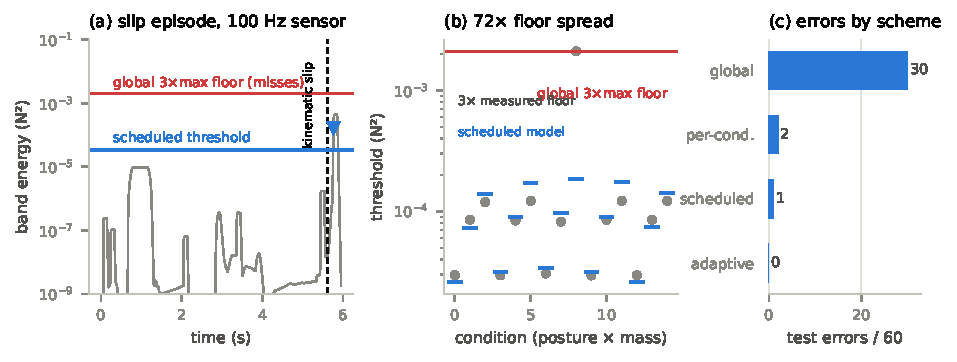
\includegraphics[width=\textwidth]{figs/F6_slip.pdf}
  \caption{Slip detection at scale. (a)~A slip episode: the band-energy
    burst clears its own condition's pre-slip floor by ${\ge}3.6\times$.
    (b)~The floor varies $9\times$ (ideal rate) to $72\times$ (100~Hz
    camera rate) across the 15 posture~$\times$~mass conditions, so no
    global threshold works. (c)~Errors by calibration scheme: scheduling
    the threshold over $(\phi,\theta,m)$ recovers near-perfect detection at
    both rates.}
  \label{fig:slip}
\end{figure*}

A grip-force rule wants a safety net: detect incipient slip and bump the
setpoint. The detector is deliberately simple --- band energy (15~Hz
one-pole high-pass, 100~ms window) of the tangential force
$\lVert (f_2, f_3) \rVert$, thresholded --- and is evaluated against
kinematic ground truth (drift $> 2$~mm; incipient slip = tangential sliding
$> 5$~mm/s sustained 50~ms) at both the ideal simulation rate and a 100~Hz
sample-and-hold camera-rate variant matching the physical sensor.

A pilot at a single posture scores perfectly at both rates, reproducing the
common literature result. The deployable question appears at scale. The
expanded study runs 90 episodes (45 induced-slip by force ramp-down, 45
clean holds) over 15 posture $\times$ mass conditions spanning the
envelope, split 30 train / 60 test:
\begin{itemize}
  \item \textbf{A single global threshold fails.} The pre-slip vibration
    floor varies $9\times$ (ideal) to $72\times$ (camera rate) across
    conditions. The only safe global choice --- $3\times$ the maximum
    training floor --- misses every test slip (0~TP\,/\,30~FN); even the
    oracle-best global threshold commits a false positive.
  \item \textbf{Detection itself is sound.} Within each condition, every
    slip burst clears that condition's own floor by ${\ge}3.6\times$
    (median $12\times$ ideal, $45\times$ camera rate). The broken piece is
    \emph{calibration transfer} across conditions
    (Fig.~\ref{fig:slip}a,b).
\end{itemize}

\textbf{Scheduled threshold.} Fit $\log_{10}$(pre-slip floor) over
$(\phi,\theta,m)$ on the training episodes --- the same scheduling recipe
as the grip-force rule --- and set the threshold to $3\times$ the predicted
floor at the current posture and load. The floor model is modest
($R^2 = 0.48$ ideal, 0.68 camera rate) but the ${\ge}3.6\times$ burst
margin absorbs the prediction error (Table~\ref{tab:slip}). This matches
the oracle-best global threshold while requiring only signals the
controller already has (Fig.~\ref{fig:slip}c). A model-free adaptive
variant --- a running-floor self-normalization guarded by an absolute
sensor-noise term and post-grasp arming --- reaches a perfect 30/0/0/30 on
this test set at both rates; its construction, ablations (each guard is
necessary), and tuning are documented in the released code. Per-condition
calibration (28/0/2/30) remains a diagnostic upper bound but assumes
training data at every operating condition --- precisely the assumption
scheduling removes.

\begin{table}[t]
  \caption{Scheduled-threshold slip detection on the 60-episode test set
    (30 slip, 30 clean-hold). UB = 95\,\% upper bound.}
  \label{tab:slip}
  \centering
  \setlength{\tabcolsep}{3pt}
  \resizebox{\columnwidth}{!}{%
  \begin{tabular}{lccccccc}
    \toprule
    rate & TP & FP & FN & TN & latency & miss (UB) & FP (UB) \\
    \midrule
    ideal (1~kHz) & 30 & 1 & 0 & 29 & 0.168~s & 0\,\% (10\,\%) &
      3.3\,\% (${\approx}13$\,\%) \\
    camera (100~Hz) & 30 & 1 & 0 & 29 & 0.170~s & 0\,\% (10\,\%) &
      3.3\,\% (${\approx}13$\,\%) \\
    \bottomrule
  \end{tabular}}
\end{table}

Camera-rate operation costs essentially nothing: the floor \emph{spread}
worsens but burst separability \emph{improves}, because sample-and-hold
decimation suppresses the broadband floor more than the slip burst.

\section{Carried Grasps and the Time Dimension}
\label{sec:carried}

\begin{figure}[t]
  \centering
  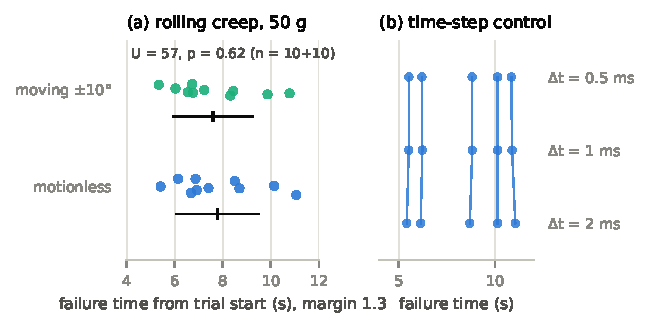
\includegraphics[width=\columnwidth]{figs/F5_creep.pdf}
  \caption{(a)~Creep failure-time distributions at margin 1.3: motionless
    vs.\ carried holds, 10 seeds each; we detect no difference
    (Mann--Whitney $U = 57$, $p = 0.62$). (b)~Time-step control: 1~ms and
    0.5~ms steps reproduce each seed's failure time to within 0.04~s.}
  \label{fig:creep}
\end{figure}

\textbf{The boundary is hold-duration-dependent.} Carrying the 50~g box
through a grasp tilt sinusoid ($\pm 10^\circ$, 0.15~Hz, 2 cycles) at
$1.3\times\fstar$ fails --- and so does a motionless hold at the same
force. With 10 seeds per condition, margin 1.3 fails 20/20 runs, and the
failure time is a distribution, not a constant: 5.4--11.1~s motionless
($7.8 \pm 1.7$~s) versus 5.3--10.8~s moving ($7.6 \pm 1.6$~s), measured
from trial start; the hold itself begins ${\approx}1.2$~s in, so these are
4--10~s of unsupported hold (Fig.~\ref{fig:rolling}'s example fails 4.3~s
into its hold). We detect no
difference between the motionless and carried distributions (Mann--Whitney
$U = 57$, $p = 0.62$; with $n = 10$ per group only large differences would
be detectable; Fig.~\ref{fig:creep}a), and the failure times are
insensitive to carry amplitude --- the motion is not what kills the grasp.
The mechanism is the same slow rolling creep of Fig.~\ref{fig:rolling}: a
grasp that passes any fixed-duration stability test just above $\fstar$
still escapes on the 5--11~s scale. Rolling creep produces almost no
tangential vibration until roll-off is imminent, so utilization monitoring
gives no warning and a vibration reflex fires too late --- no detector can
rescue a grasp commanded at margin 1.3.

\begin{figure}[t]
  \centering
  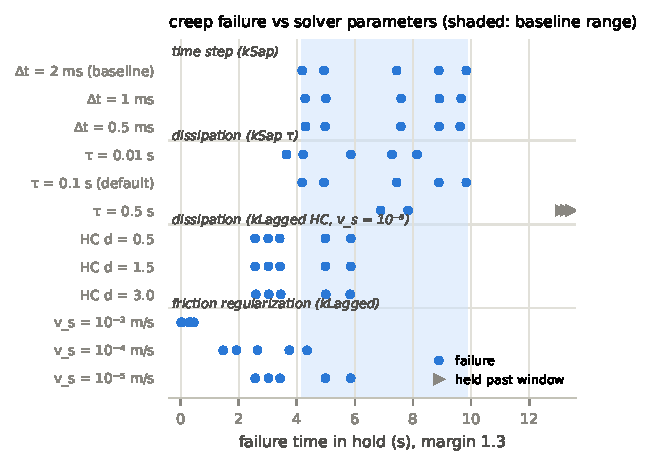
\includegraphics[width=\columnwidth]{figs/F8_sensitivity.pdf}
  \caption{Failure time of the margin-1.3 motionless hold under every
    solver parameter that could have manufactured the creep (5 seeds per
    condition; shaded band: baseline seed range). Time step, Kelvin--Voigt
    relaxation time $\tau$ near default, and Hunt--Crossley dissipation
    (live under \texttt{kLagged}) leave the distribution in the baseline
    band; only macroscopically sloppy friction regularization
    ($v_s = 10^{-3}$~m/s) changes the picture, and tightening it
    saturates. No condition eliminates the failure.}
  \label{fig:sens}
\end{figure}

\textbf{The creep is physics, not a solver artifact.} Because the solver's
own approximations could in principle manufacture a slow creep --- a
viscous timescale from the contact dissipation, or residual slip from
regularized friction --- we varied both, plus the discrete contact
approximation itself, on the margin-1.3 motionless hold
(Fig.~\ref{fig:sens}; 5 seeds per condition). (i)~\emph{Time step:}
1~ms and 0.5~ms steps reproduce each seed's failure time to within 0.04~s
(Fig.~\ref{fig:creep}b); under \texttt{kSap} this also bounds the friction
regularization, whose residual creep velocity scales with the step.
(ii)~\emph{Dissipation:} varying the Hunt--Crossley dissipation
$3\times$ in either direction (under \texttt{kLagged}, where it is
consumed) leaves mean failure time unchanged to within 0.01~s; reducing
the \texttt{kSap} Kelvin--Voigt relaxation time $10\times$ below default
shifts it only $-15\,\%$. Dissipation does not manufacture the creep ---
raising $\tau$ to an unphysically viscous 0.5~s \emph{retards} it (3/5
seeds outlast the 14.3~s window), so the baseline errs conservative: a
more elastic contact fails at least as fast. (iii)~\emph{Friction
regularization:} under \texttt{kLagged}/\texttt{kSimilar}, whose
regularized friction is set directly by the stiction tolerance $v_s$, a
sloppy $v_s = 10^{-3}$~m/s fails immediately (macroscopic regularization
slip), but failure times \emph{saturate} as $v_s$ tightens ($10^{-4} \to
10^{-5}$~m/s moves the mean only 28\,\% for a $10\times$ change) --- and
the failure never disappears. The phenomenon and its timescale are
robust; the exact seconds carry a ${\sim}1.6\times$ spread between
contact approximations (means 5.2~s \texttt{kLagged} vs.\ 8.3~s
\texttt{kSap} from trial start), which is one reason the design rule
below is a force margin, not a timed allowance.

\textbf{Design rule.} Command
$f_1 = 2.0 \times (mg/2)/\mueff$
for sustained holds and slow manipulation with the rolling DOF
unregulated (\S\ref{sec:closedloop} lowers this to
${\approx}1.3\times$ under active rolling regulation). At this margin, 30/30 seeded
carry runs (10 seeds $\times$ three controllers --- fixed force,
map-scheduled, scheduled + vibration reflex) complete the full posture
sweep with ${\le}0.85$~mm drift. The 1.3 margin is trustworthy only on
the timescale of the 3~s acceptance window itself: the earliest observed
creep failure is 4.1~s of hold at baseline, and 2.6~s under the
alternative contact approximation. Along the
tested trajectory the fitted $\mueff$ is nearly flat in tilt --- consistent
with \S\ref{sec:envelope}'s flatness result --- so scheduling
${\approx}$~fixed force by design there; the scheduled controller earns its
keep in excursions that change PIP flexion or approach regime boundaries.
(Phase-B forces were commanded from a pre-revision fit; under the final
equation the same 0.75~N is margin ${\approx}2.1$ and the failing 0.49~N is
margin ${\approx}1.4$ --- conclusions unchanged.)

\section{Closing the Loop on the Rolling DOF}
\label{sec:closedloop}

Everything above servos a constant squeeze force with nothing regulating
the rolling degree of freedom --- while the controllers of
\cite{psomopoulou2018stable,psomopoulou2021pinching} regulate exactly that
DOF. What does active rolling regulation buy in minimal grip force? To
our knowledge this has not been measured. We add to the testbed a
simplified tactile analogue of rolling-orientation control: the object's
pitch about the lateral axis is observed as the \emph{antisymmetric
vertical migration of the two contact centroids} in the tip frames ---
a signal available from the idealized TacTip reading alone --- and both
domes are rolled to follow it through a rate-limited differential PIP
reference trim ($k_p = 10^3$~rad/m on the filtered 5~Hz error, trim
clamped to $\pm 0.25$~rad at 0.7~rad/s; sign and gain from a margin-1.3
tuning study --- arrest appears at $k_p \gtrsim 300$ and plateaus by
$10^3$).

\textbf{Regulation arrests the creep.} The margin-1.3 motionless hold
that fails 20/20 open-loop (\S\ref{sec:carried}) survives 10/10 seeded
14.3~s windows with regulation on, with total rotation pinned at
$\le 1.6^\circ$ (versus a $176^\circ$ tumble). Probing lower: 5/5 seeds
hold at margin 1.15 and 3/5 at margin 1.05. The sustained-hold
requirement drops from the measured $\times 2.0$ to
${\approx}\times 1.15$ --- a 42\,\% force saving for long holds.

\textbf{But the boundary itself does not move.} Re-bisecting $\fstar$
with regulation active (5 seeds, reference posture) gives
0.216\,/\,0.417\,/\,0.539~N at 30\,/\,50\,/\,60~g versus
0.209\,/\,0.435\,/\,0.577~N open-loop: $-3$ to $+7$\,\% in $\mueff$,
inside the audit's seed noise. The 3~s acquisition boundary is
control-invariant for this regulator.

\textbf{Reading.} The rolling discount has two parts. The static floor
--- whether a pinch equilibrium exists at all on the 3~s scale --- is
set by patch geometry and is not recovered by rolling the tips faster
than the object escapes. What control removes is the \emph{time
dimension}: under regulation the sustained-hold requirement collapses
onto the acquisition boundary itself
($(mg/2)/(1.15\,\fstar) \approx \mueff$), so the $\times 2.0$ margin of
\S\ref{sec:carried} is revealed as the price of leaving the rolling DOF
open-loop, not a property of the boundary. For the set-point law this
means: command $\times 2.0$ without rolling regulation, and
${\approx}\times 1.3$ (10/10 here) with it. The gains are tuned for this
envelope; a stability analysis of the regulator belongs to the
rolling-control theory this section borrows from.

\section{Limitations and Conclusion}
\label{sec:limitations}

\textbf{Limitations.} (i)~The tactile signal is an idealized TacTip --- the
hydroelastic contact resultant and centroid; real marker-flow force
estimates add noise, hysteresis, and calibration error. The 100~Hz variant
bounds only the rate effect. Hardware validation, following the sim-to-real
path demonstrated for TacTip-class sensors \cite{lin2022tactilegym2}, is
the natural next step. (ii)~Boundary trials at 2~ms Nyquist-limit vibration
content to 250~Hz; slip trials use 1~ms. (iii)~The 2~mm~/~3~s stability
criterion itself defines $\fstar$, and \S\ref{sec:carried} shows the
boundary moves with hold duration; $\fstar$ values are tied to that window
(the $\times 2.0$ rule is the duration-robust statement). (iv)~Sweep
boundaries use 2 seeds per probe and are seed-limited at 60~g (spread to
32\,\%); the shape/material tables and carry statistics use 5 and 10 seeds.
(v)~A perfect 30~+~30 slip score still only bounds each error rate below
${\sim}10\,\%$ (rule of three); the floor model and adaptive constants are
tuned to this hand/object envelope. (vi)~One grasp width (25~mm) and one
base material pair; masses validated 30--60~g; the material study gives
scaling to other pairs only at the reference posture.

\textbf{Conclusion.} For soft tactile fingertips, the minimal-grip-force
question is not a friction question. In this simulation study the
stability boundary is set by rolling: the interface stays in stick while
the patch migrates, the boundary binds 25--35\,\% below the Coulomb limit
at every friction tested, moves $2\times$ with shape at fixed friction,
worsens as solid domes soften, and --- near the boundary --- depends on
how long you intend to hold, robustly to the solver's own dissipation and
regularization parameters. All of this is invisible to a friction-cone
analysis and all of it is capturable: a one-line mass-dependent
calibration with a measured envelope predicts held-out boundaries 16/16,
a posture-scheduled threshold makes a simple vibration detector usable at
the sensor's real frame rate, a $\times 2.0$ margin converts the rule
into a controller that did not drop an object in 30 seeded carries, and
closing the loop on the rolling degree of freedom itself arrests the
creep that made the margin necessary. This paper contributes that
measured map --- the flat-in-posture $\mueff$, the support and fragile
regimes, the sensitivity--stability trade-off --- and the calibration
recipe distilled from it, with every number reproducible from the
released code and data; hardware validation on physical TacTips is the
next step.

\balance
\bibliographystyle{IEEEtran}
\bibliography{refs}

\end{document}
